\documentclass[18pt]{beamer}
\usetheme{Madrid}

\usepackage{graphics}


\newcommand{\centeredlargetext}[3]{
{
\setbeamertemplate{navigation symbols}{}
\setbeamercolor{background canvas}{bg={#1}}
\color{#2}
\begin{frame}[plain]
\fontsize{36pt}{36pt}\selectfont
\center
\begin{center}
{#3}
\end{center}
\end{frame}
}}


\begin{document}

\title[Open Source]{Open Source Software Practices}
\subtitle[UH]{University of Houston}
\author[Luis Ibanez]{Luis Ibanez}
\institute[Kitware]{KITWARE Inc.\\
Clifton Park, NY
}
\date[April 2011]{April 6 2011}

\begin{frame}
\titlepage
\end{frame}


{
\setbeamertemplate{navigation symbols}{}
\begin{frame}[plain]
\center
\begin{center}
This presentation is copyrighted by\\
The \textbf{Insight Software Consortium}\\
\bigskip
distributed under the\\
\textbf{Creative Commons by Attribution License 3.0}\\
\url{http://creativecommons.org/licenses/by/3.0}\\
\bigskip
Images used in this presentation are attributed in the last slide.
\end{center}
\end{frame}
}


\begin{frame}
  \tableofcontents
\end{frame}


{
\setbeamertemplate{navigation symbols}{}
\setbeamertemplate{background canvas}{
  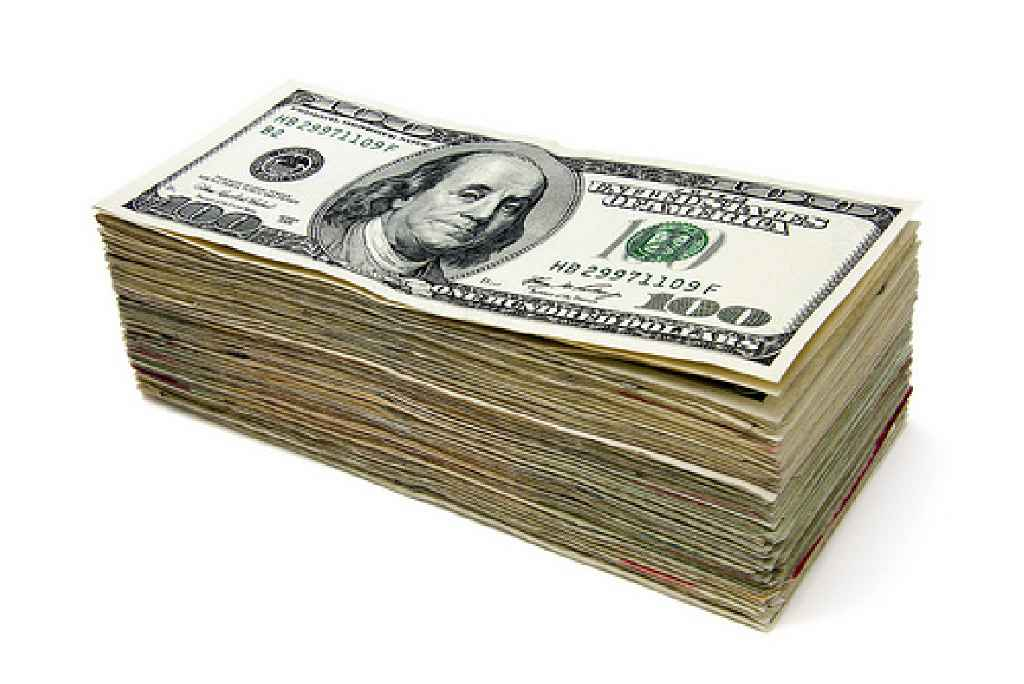
\includegraphics[width=\paperwidth,height=\paperheight]{../Art/3366720659_small.jpg}
}
\begin{frame}[plain]
\end{frame}
}


\part{Economics}

\centeredlargetext{white}{black}{
Economics
}

\section{Manufacturing Delusion}

\centeredlargetext{black}{white}{
The Software\\
Manufacturing\\
Delusion
}


\begin{frame}[plain]
\fontsize{18pt}{18pt}\selectfont
\center
\begin{quote}
Software is largely a \textbf{service} industry\\
\pause
operating under the persistent\\
\pause
but unfounded \textbf{delusion}\\
\pause
that it is a \textbf{manufacturing} industry.\\
\pause
\end{quote}
\bigskip
\begin{flushright}
Eric S. Raymond
\end{flushright}
\end{frame}


{
\setbeamertemplate{navigation symbols}{}
\setbeamertemplate{background canvas}{
  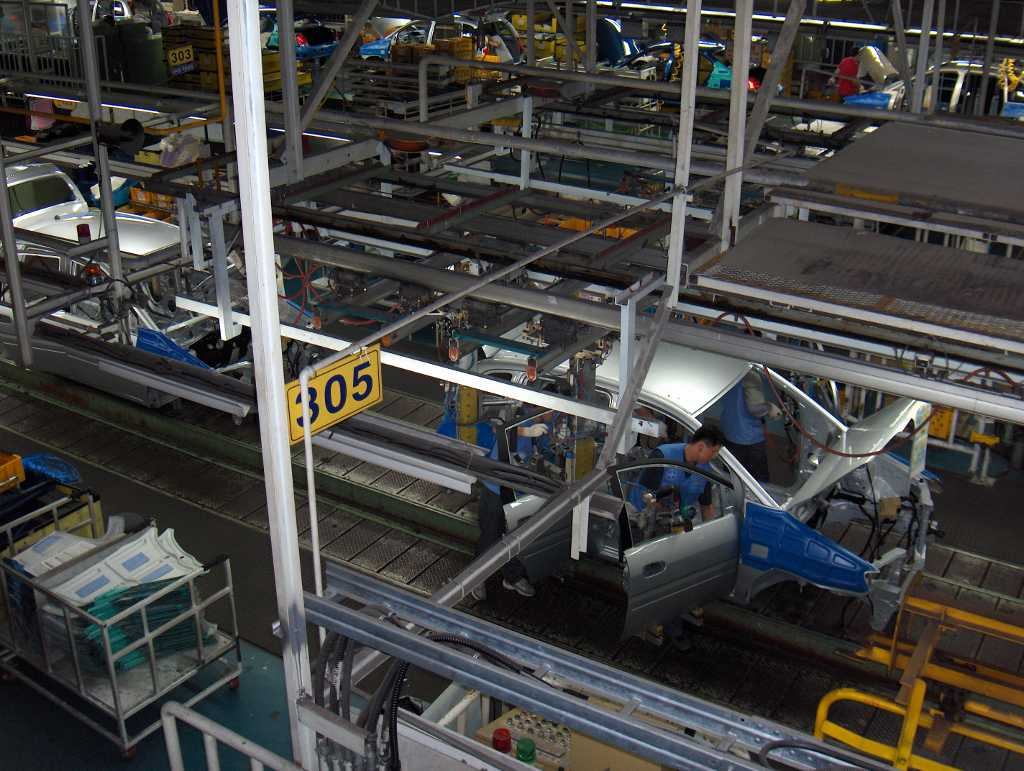
\includegraphics[width=\paperwidth,height=\paperheight]{../Art/Hyundai_car_assembly_line_scaled.jpg}
}
\begin{frame}[plain]
\end{frame}
}


{
\setbeamertemplate{navigation symbols}{}
\setbeamertemplate{background canvas}{
  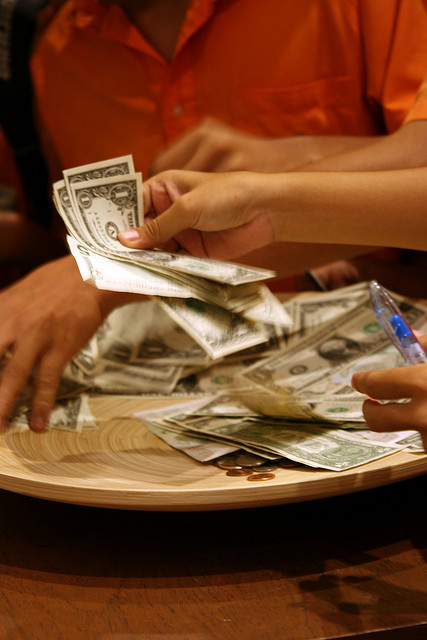
\includegraphics[width=0.55\textwidth,height=\paperheight]{../Art/2672465894_5b21e12135_z.jpg}
  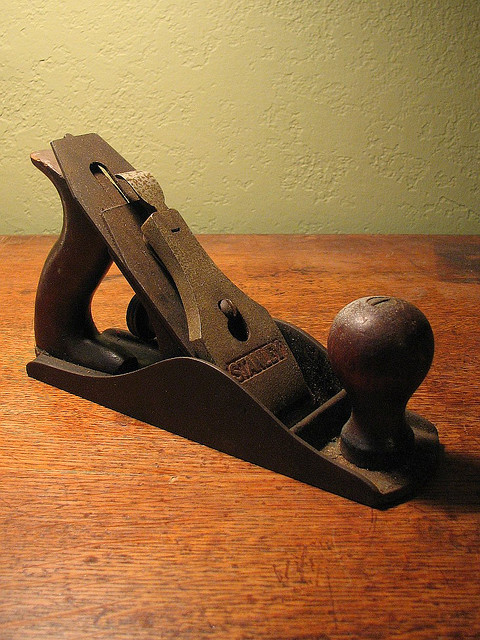
\includegraphics[width=0.55\textwidth,height=\paperheight]{../Art/4293485922_7474ef04ce_z.jpg}
  }
\begin{frame}
\frametitle{FIXME: Sale Value vs Use Value}
Insert here an image of a Software Box (to convey the idea of a product)
\end{frame}
}


{
\setbeamertemplate{navigation symbols}{}
\setbeamertemplate{background canvas}{
  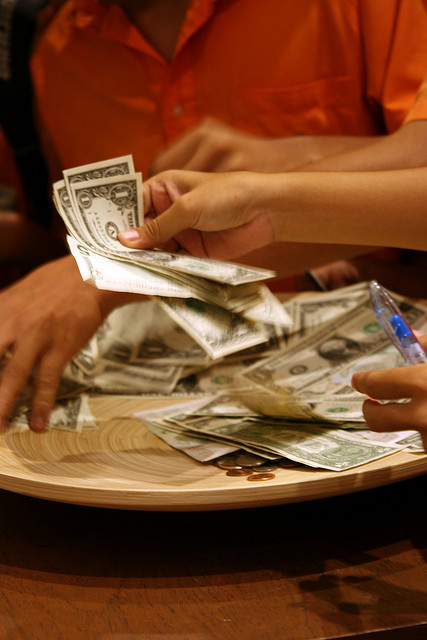
\includegraphics[width=0.55\textwidth,height=\paperheight]{../Art/2672465894_5b21e12135_z.jpg}
  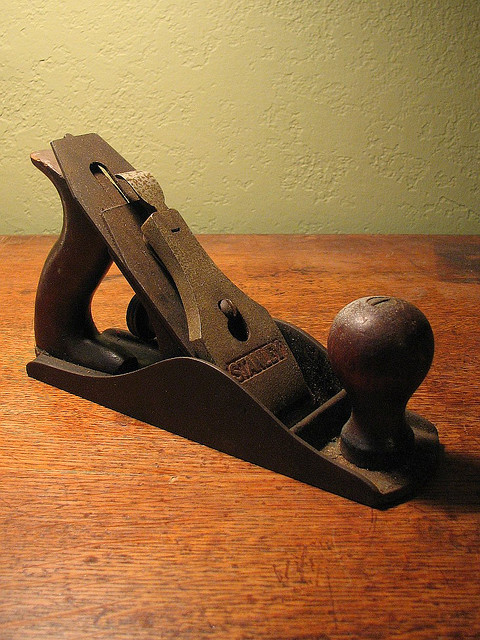
\includegraphics[width=0.55\textwidth,height=\paperheight]{../Art/4293485922_7474ef04ce_z.jpg}
  }
\begin{frame}
\frametitle{Sale Value vs Use Value}
\end{frame}
}


{
\setbeamertemplate{navigation symbols}{}
\begin{frame}
\frametitle{Largest Software Publishers - 2010}

\begin{center}
\begin{tabular}{clrrr}
\hline
  \textbf{Rank
\footnote{
\url{http://www.softwaretop100.org/global-software-top-100-edition-2010}}
} &\textbf{Publisher} &	\textbf{Software \$M} & \textbf{Total \$M} & \textbf{Percent} \\
\hline
\hline
1 &  \textbf{Microsoft} & 49,090  & 61,159 &  80\% \\
2 &  \textbf{IBM} & 21,396  & 95,758  & 22\% \\
3 &  \textbf{Oracle} & 18,582  & 22,734 &  82\% \\
4 &  SAP & 11,368  & 15,373 &  74\% \\
5 &  Ericsson & 7,595  & 29,014 &  26\% \\
6 &  Nintendo & 6,799  &  17,762 &  38\% \\
7 &  HP & 6,183  &  116,245 &  5\% \\
8 &  \textbf{Symantec} & 5,565  & 5,992 &  93\% \\
9 &  Nokia Siemens & 4,529  &  18,114 &  25\% \\
10&  Blizzard & 4,279  & 4,279 & 100\% \\
\end{tabular}

\end{center}
\end{frame}
}


{
\setbeamertemplate{navigation symbols}{}
\begin{frame}
\frametitle{Largest Software Publishers - 2010}

\begin{center}
\begin{tabular}{clrrr}
\hline
\textbf{Rank
\footnote{
\url{http://www.softwaretop100.org/global-software-top-100-edition-2010}}
} &\textbf{Publisher} &	\textbf{Software \$M} & \textbf{Total \$M} & \textbf{Percent} \\
\hline
\hline
11 & CA & 4,012  & 4,318 & 93\% \\
12 & EMC & 3,960  & 14,026 & 28\% \\
13 & \textbf{Electronic Arts} & 3,728  &  3,728 & 100\% \\
14 & \textbf{Adobe} & 2,796 &  2,987 & 94\% \\
15 & Cisco & 2,137 & 36,633 & 6\% \\
16 & SunGard & 1,996  & 5,508 & 36\% \\
17 & Sony & 1,914 &  79,441 & 2\% \\
18 & BMC & 1,758& 1,888 & 93\% \\
19 & Alcatel-Lucent & 1,635  &  21,835 & 8\% \\
20 & Konami & 1,594 &  2,887 & 55\% \\
\end{tabular}

\end{center}
\end{frame}
}


{
\setbeamertemplate{navigation symbols}{}
\begin{frame}
\frametitle{Largest Software Publishers - 2010}

\begin{center}
\begin{tabular}{clrrr}
\hline
\textbf{Rank
\footnote{
\url{http://www.softwaretop100.org/global-software-top-100-edition-2010}}
} &\textbf{Publisher} &	\textbf{Software \$M} & \textbf{Total \$M} & \textbf{Percent} \\
\hline
\hline
21 & Hitachi & 1,589 & 99,818 & 2\% \\
22 & Dassault & 1,584 & 1,803 & 88\% \\
23 & Infor & 1,575 & 2,100 & 75\% \\
24 & Sage & 1,557 & 2,336 & 67\% \\
25 & \textbf{Autodesk} & 1,557 & 1,764 & 88\% \\
\ldots & \ldots & \ldots & \ldots & \ldots \\
28 & \textbf{Apple} & 1,218 &	43,086 & 	\textbf{3\%}  \\
32 & SAS Institute & 1,155 	& 	2,310 &	50\%  \\
37 & VMWare & 1,029 &	2,024 & 	51\%  \\
39 & McAfee & 964 &	1,927 & 50\% \\
\end{tabular}

\end{center}
\end{frame}
}


\begin{frame}
\frametitle{Distribution of Software Publisher Size}
  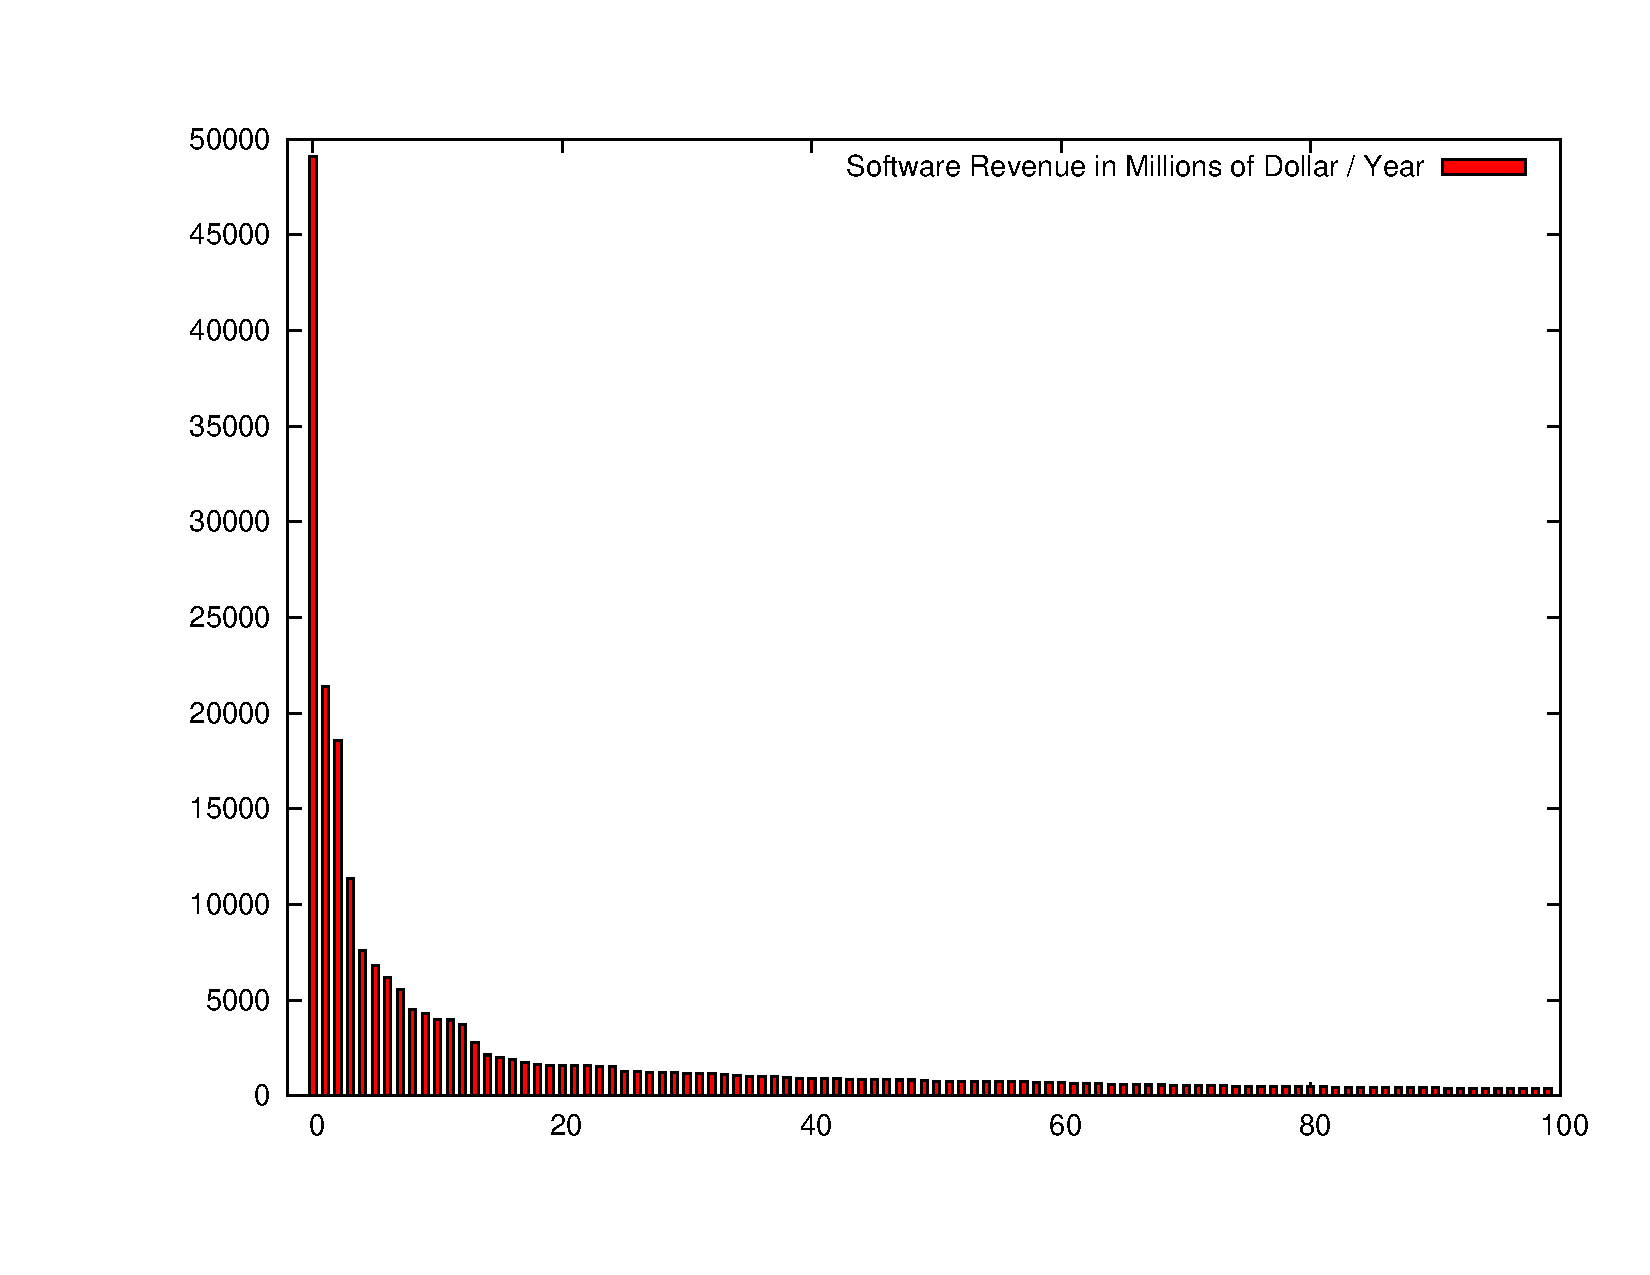
\includegraphics[width=0.9\textwidth,height=0.9\paperheight]{../Art/LargestSoftwarePublishersPlot.pdf}
\end{frame}


\begin{frame}
\frametitle{Size of the Software Publishing Industry - 2010}
\fontsize{72pt}{90pt}\selectfont
\begin{center}
\$ 221 Billion
\end{center}
\end{frame}


\begin{frame}
\frametitle{Some Notable Companies}

\begin{tabular}{lrrr}
\hline
\textbf{Publisher} &	\textbf{Annual Revenue} & \textbf{Cost of Revenue} & \textbf{Gross Profit} \\
\hline
\hline
\href{http://www.google.com/finance?fstype=ii\&q=NASDAQ:MSFT}{Microsoft Corp.}	& \$ 62,484 M & \$ 12,395 M  & \$ 50,089 M  \\
\hline
\href{http://www.google.com/finance?q=NYSE:IBM\&fstype=ii}{IBM Corp.} & \$ 95,759 M & \$ 51,972 M & \$ 43,787 M \\
\hline
\href{http://www.google.com/finance?q=NASDAQ:AAPL\&fstype=ii}{Apple Inc.} & \$ 42,905 M & \$ 25,683 M & \$ 17,222 M \\
\hline
\href{http://www.google.com/finance?q=NASDAQ:ORCL\&fstype=ii}{Oracle} & \$ 26,820 M & \$ 5,764 M & \$ 21,056 M \\
\hline
\href{http://www.google.com/finance?q=NASDAQ:SYMC\&fstype=ii}{Symantec}	&	\$ 5,985 M & \$ 1,105 M & \$ 4,880 M \\
\hline
\href{http://www.google.com/finance?q=NASDAQ:ADBE\&fstype=ii}{Adobe} & \$ 943 M & \$ 107 M & \$ 835 M \\
\hline
\end{tabular}

\bigskip
\begin{center}
Balance Sheets - September 2009 - September 2010
\end{center}

\end{frame}


{
\setbeamertemplate{navigation symbols}{}
\setbeamertemplate{background canvas}{
  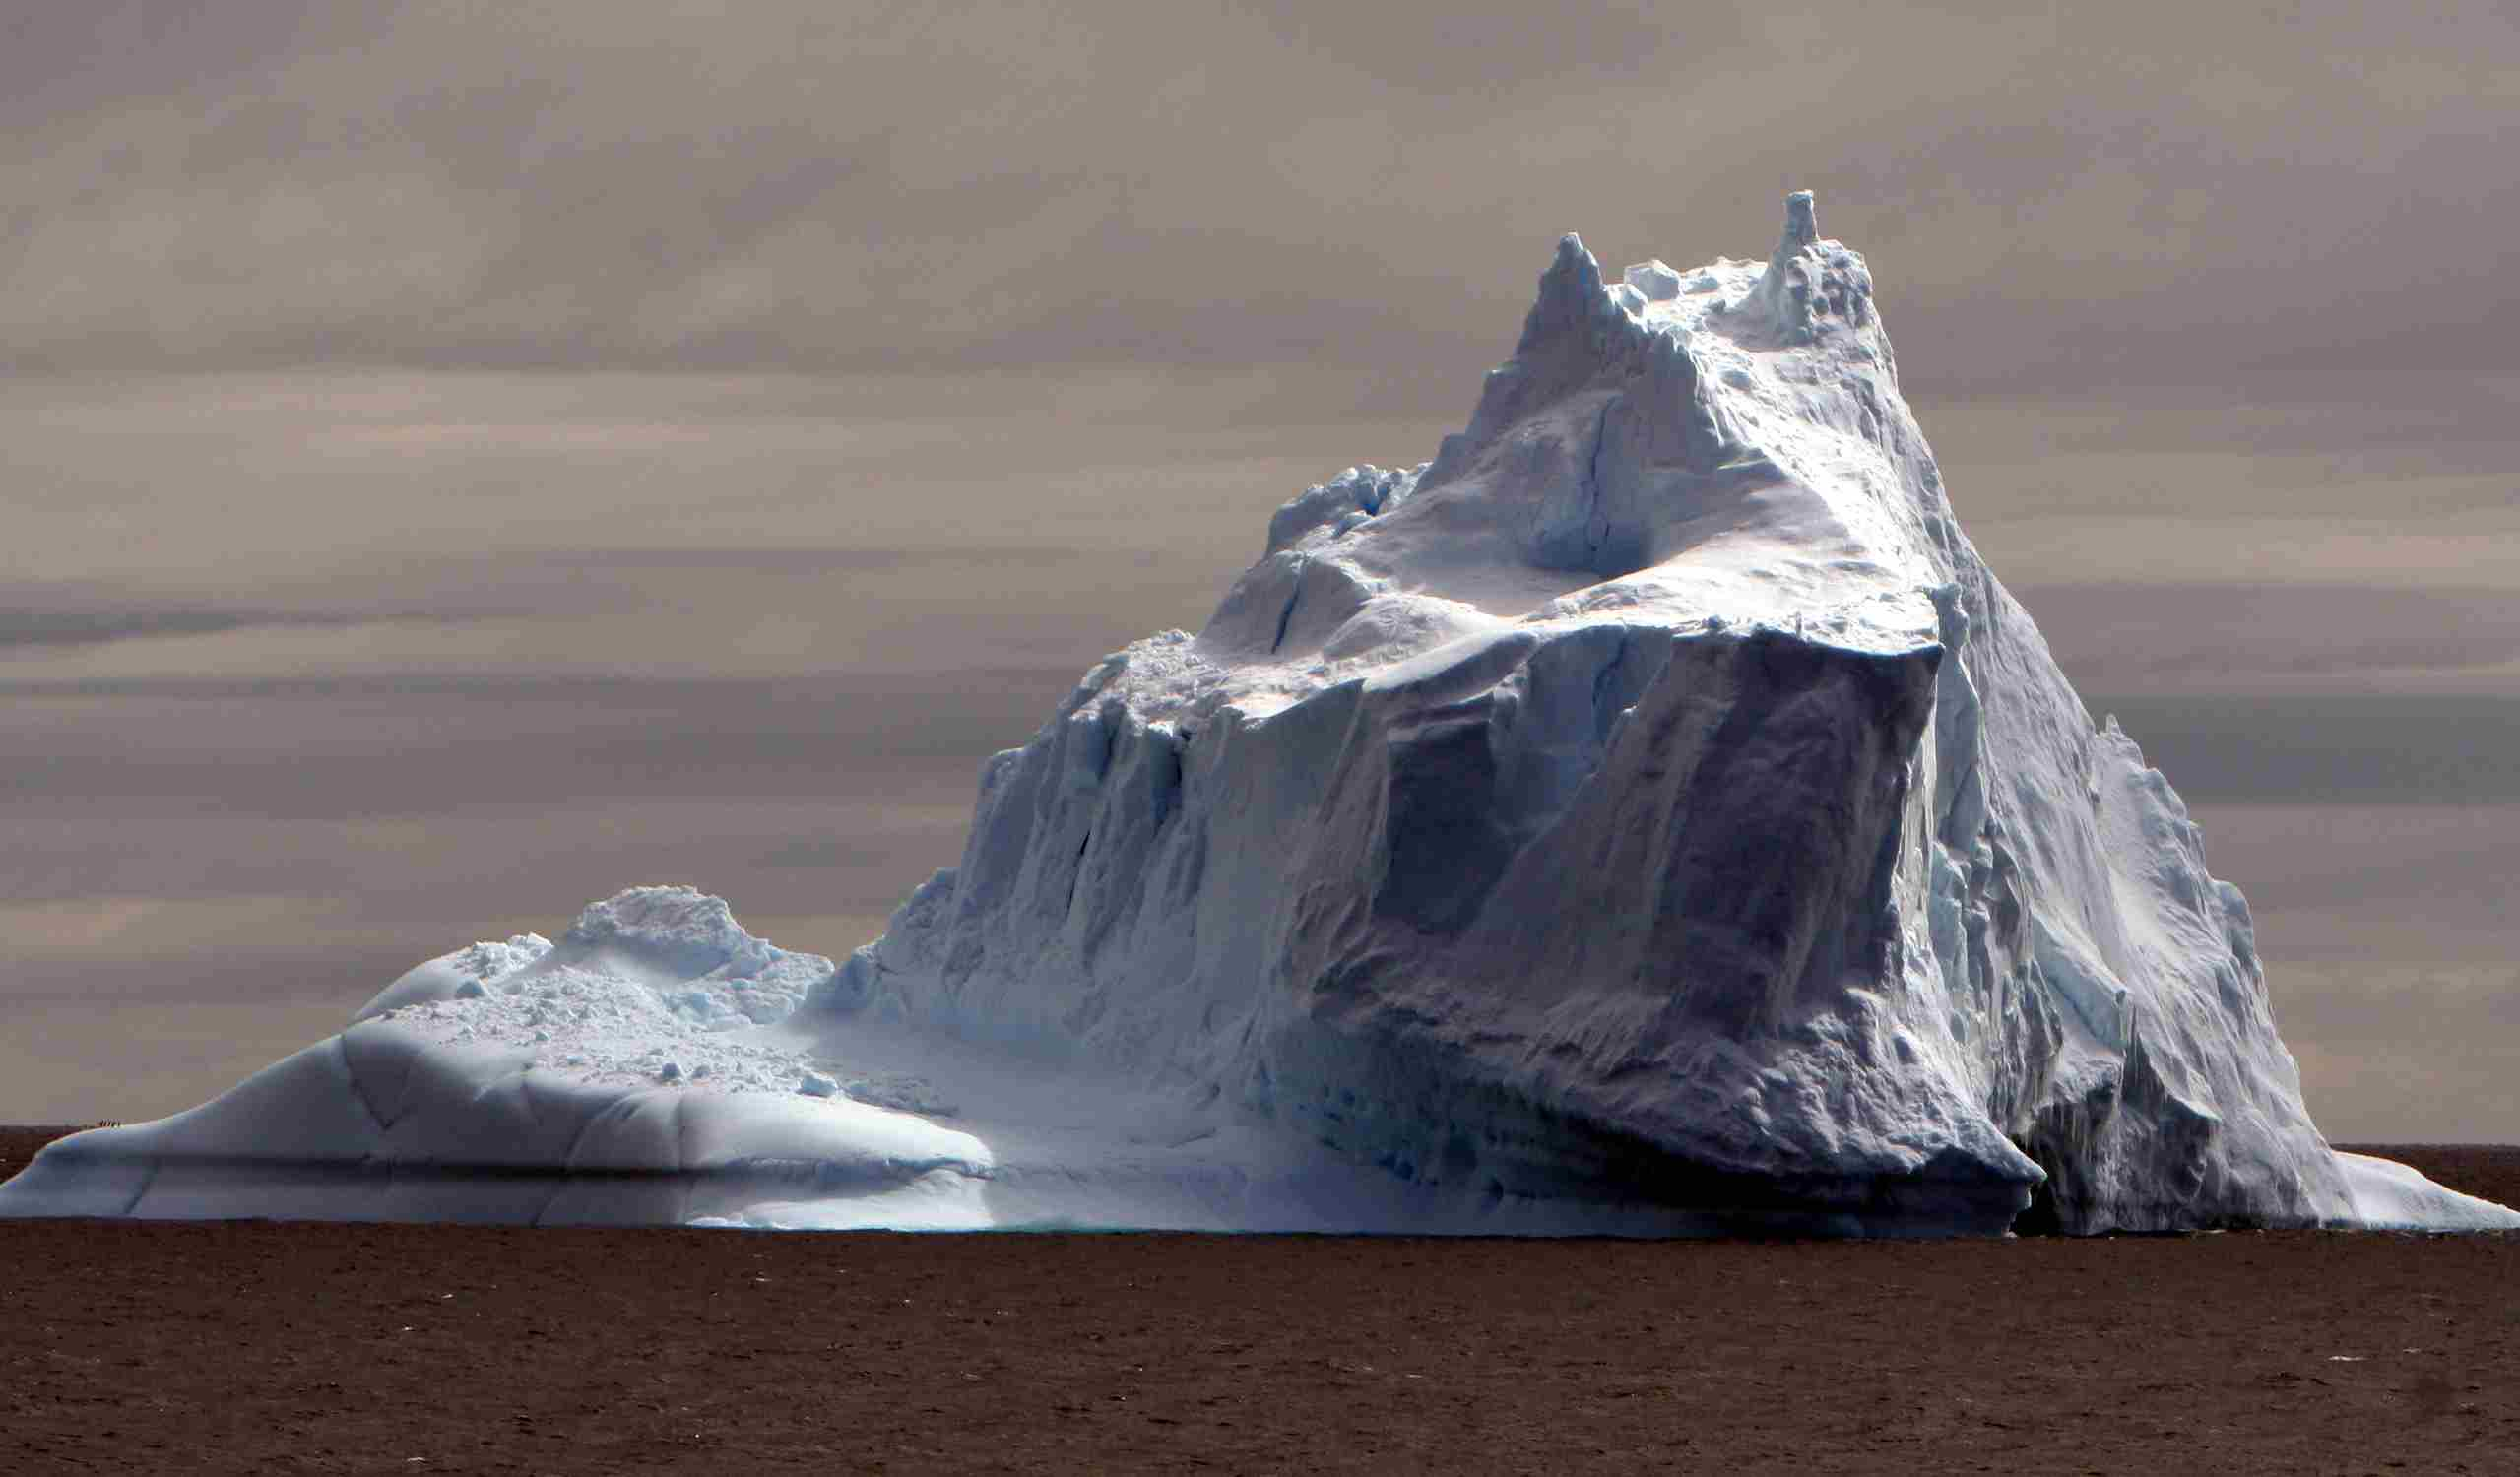
\includegraphics[width=\paperwidth,height=\paperheight]{../Art/Iceberg_Antarctica_Crop.jpg}
}
\begin{frame}[plain]
\end{frame}
}


{
\setbeamertemplate{navigation symbols}{}
\begin{frame}
\frametitle{Apple Inc.}

\begin{center}
\begin{tabular}{lrr}
\hline
\textbf{Product}
\footnote{
\href{http://phx.corporate-ir.net/External.File?item=UGFyZW50SUQ9NzgwODJ8Q2hpbGRJRD0tMXxUeXBlPTM=&t=1}
{Financial Report, First Quarter 2011, page 25:}
 \url{http://www.apple.com/investor/} }
& \textbf{Sales \$M}
& \textbf{Percent} \\
\hline
\hline
\textbf{iPhone} and services & \textbf{10,468} &  39.15\%  \\
iPad and services & 4,608 & 17.23\% \\
Laptops & 3,699 & 13.83\% \\
iPod & 3,425 & 12.81\% \\
Desktops & 1,731 & 6.47\% \\
Music and services & 1,431 & 5.35\%  \\
\textbf{Software} and others &  786 & \textbf{2.94\%} \\
Perihelias &  593 & 2.22\% \\
\hline
Total &  26,741 & 100\% \\
\end{tabular}

\end{center}
\end{frame}
}


\centeredlargetext{white}{black}{
\$ 13 Trillion
}


\begin{frame}[plain]
\fontsize{30pt}{30pt}\selectfont
\center
\begin{quote}
Finished products\\
are for decadent minds
\end{quote}
\bigskip
\fontsize{18pt}{18pt}\selectfont
\begin{flushright}
Isaac Asimov\\
``The Foundation''
\end{flushright}
\end{frame}


{
\setbeamertemplate{navigation symbols}{}
\begin{frame}
\frametitle{Lack of Quality Control}
\center
\Huge
Inadequate\\
Software Testing Infrastructure\\
costs the U.S.
\pause
\Huge
\bigskip
\begin{center}
\textbf{\$ 60 Billion} a year\footnote{\url{http://www.nist.gov/director/prog-ofc/report02-3.pdf}}
\end{center}
\end{frame}
}


{
\setbeamertemplate{navigation symbols}{}
\begin{frame}
\frametitle{Lack of Quality Control}
\Huge
\begin{center}
\textbf{\$ 0.2\%} of GDP
\end{center}
\end{frame}
}


{
\setbeamertemplate{navigation symbols}{}
\begin{frame}
\frametitle{Lack of Quality Control}
\Huge
\begin{center}
\textbf{Twice the NIH Budget}
\end{center}
\end{frame}
}



\begin{frame}[plain]
\frametitle{Sale Value versus Use Value}
  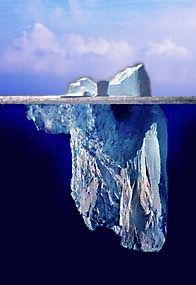
\includegraphics[width=0.5\textwidth,height=\paperheight]{../Art/Iceberg.jpg}
\end{frame}


{
\setbeamertemplate{navigation symbols}{}
\setbeamertemplate{background canvas}{
  
\includegraphics[width=\paperwidth,height=\paperheight]{../Art/osi_symbol.png}
}
\begin{frame}[plain]
\end{frame}
}


\centeredlargetext{black}{white}{
The Tragedy\\
of the\\
Commons\\
}


\begin{frame}
\frametitle{The Tragedy of the Commons}
\Huge
\begin{itemize}
\item \textbf{Multiple} Individuals
\pause
\item Acting \textbf{Rationaly}
\pause
\item Driven by \textbf{Self-Interest}
\pause
\item Sharing a \textbf{common} resource
\end{itemize}
\end{frame}


{
\setbeamertemplate{navigation symbols}{}
\setbeamertemplate{background canvas}{
  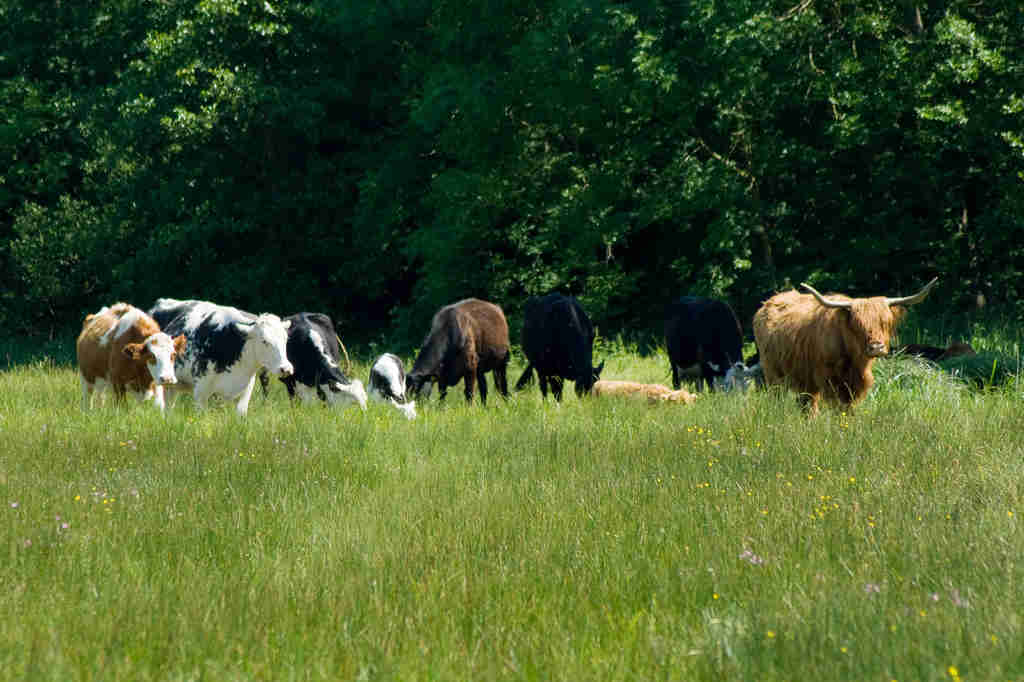
\includegraphics[width=\paperwidth,height=\paperheight]{../Art/4924182750_f128706196_b_smaller.jpg}
}
\begin{frame}[plain]
\end{frame}
}


\centeredlargetext{black}{white}{
The\\
Over-Exploitation\\
Problem
}


\begin{frame}
\frametitle{The Tragedy of the Commons - Ambiguity}
\Huge
\begin{itemize}
\item Common Property Resources
\pause
\item Open Access Resources
\end{itemize}
\end{frame}


\centeredlargetext{black}{white}{
Rival Goods
}


{
\setbeamertemplate{navigation symbols}{}
\setbeamertemplate{background canvas}{
  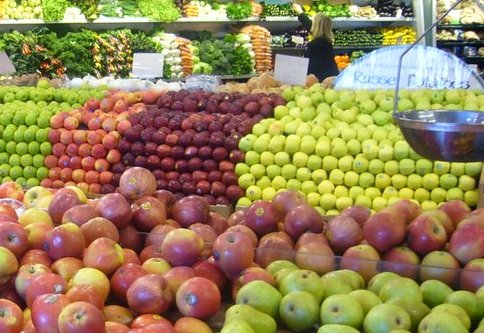
\includegraphics[width=\paperwidth,height=\paperheight]{../Art/Apples_supermarket_cropped.jpg}
}
\begin{frame}[plain]
\end{frame}
}


\centeredlargetext{black}{white}{
Excludable Goods
}


\centeredlargetext{black}{white}{
Public Goods
}


\centeredlargetext{black}{white}{
Common Property\\
Resources
}

\centeredlargetext{black}{white}{
Open Access\\
Resources
}


\centeredlargetext{white}{black}{
The Coordination\\
Problem
}


{
\setbeamertemplate{navigation symbols}{}
\setbeamertemplate{background canvas}{
  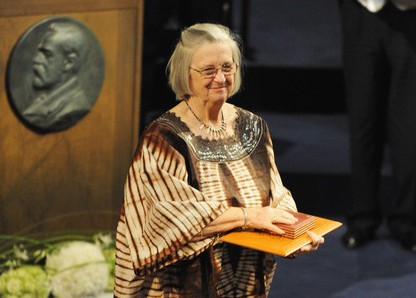
\includegraphics[width=\paperwidth,height=\paperheight]{../Art/ElinorOstromNobelPrizeCeremony2009.jpg}
}
\begin{frame}[plain]
\end{frame}
}


\begin{frame}
\frametitle{Governance}
\Huge
\begin{itemize}
\item Fisheries
\pause
\item Forests
\pause
\item Irrigation channels
\end{itemize}
\end{frame}


\begin{frame}
\frametitle{Management of Common Pool Resources}
\Large
\begin{itemize}
\item Mountain Forest/Grazing in \textbf{Switzerland}, \textbf{500} years
\pause
\item Mountain Forest/Grazing in \textbf{Japan}, \textbf{400} years
\pause
\item Irrigation Systems in \textbf{Spain}, \textbf{1,000} years
\pause
\item Irrigation Systems in the \textbf{Philippines}, \textbf{500} years
\end{itemize}
\end{frame}


\section{Practices}

\begin{frame}
\frametitle{Governance}
\Huge
\begin{itemize}
\item Benevolent Dictator
\pause
\item Bazaar
\end{itemize}
\end{frame}


{
\setbeamertemplate{navigation symbols}{}
\setbeamertemplate{background canvas}{
  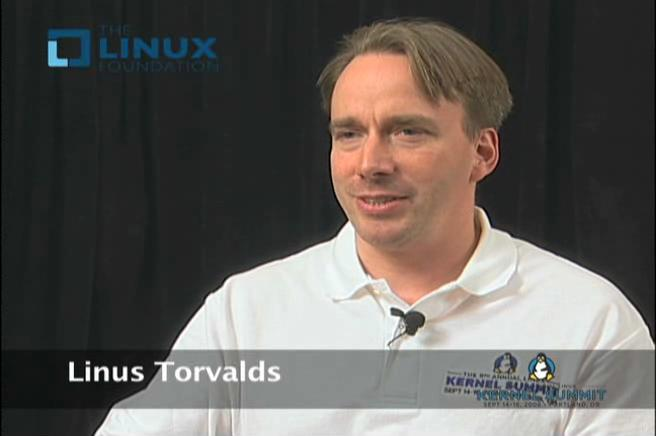
\includegraphics[width=\textwidth,height=\paperheight]{../Art/Linus_Torvalds_lks08.jpg}
}
\begin{frame}[plain]
\end{frame}
}



\centeredlargetext{black}{white}{
Free\\
Rider
}


{
\setbeamertemplate{navigation symbols}{}
\setbeamertemplate{background canvas}{
  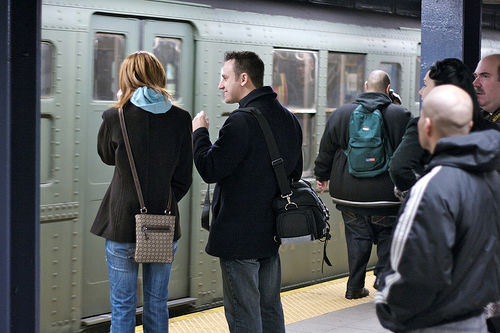
\includegraphics[width=\paperwidth,height=\paperheight]{../Art/2150546585_b3389ea99e_smaller.jpg}
}
\begin{frame}[plain]
\end{frame}
}


\centeredlargetext{black}{white}{
The Problem of\\
Commitment
}


\centeredlargetext{black}{white}{
\emph{``Nobody wants\\
to be a sucker''}
}


\centeredlargetext{black}{white}{
Conditional\\
Compliance
}

\centeredlargetext{black}{white}{
The Cost of\\
Ownership
}


{
\begin{frame}[plain]
\Huge
\center
\begin{center}
The Problem of\\
Mutual Monitoring
\end{center}
\end{frame}
}

{
\setbeamertemplate{navigation symbols}{}
\setbeamertemplate{background canvas}{
  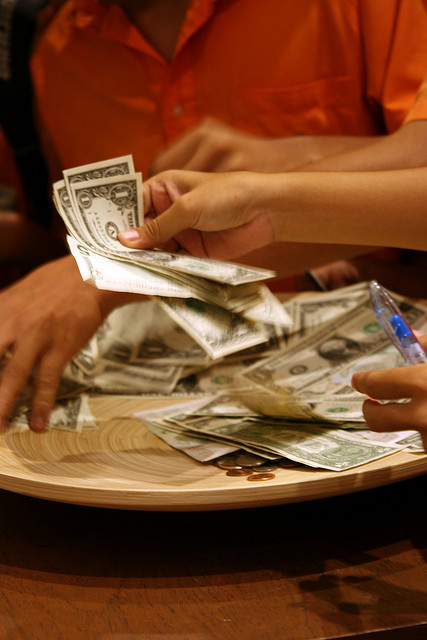
\includegraphics[width=0.55\textwidth,height=\paperheight]{../Art/2672465894_5b21e12135_z.jpg}
  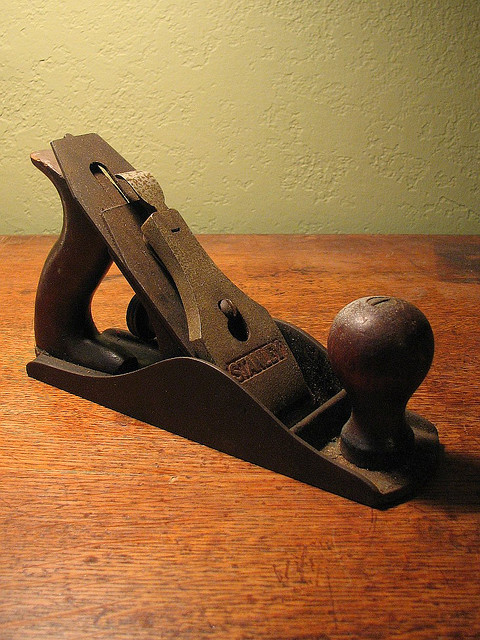
\includegraphics[width=0.55\textwidth,height=\paperheight]{../Art/4293485922_7474ef04ce_z.jpg}
  }
\begin{frame}
\frametitle{Dashboard Quality Control}
\end{frame}
}


\begin{frame}
\frametitle{Bug/Issue Trackers}
\Huge
\begin{itemize}
\item Two-Way Communication
\pause
\item Developes and Community exchange information
\pause
\item History of Bugs / Actions
\end{itemize}
\end{frame}


\begin{frame}
\frametitle{Bug/Issue Trackers}
\Huge
\begin{itemize}
\item Bug Fixing
\pause
\item Project Coordination
\pause
\item Avoid Duplication of Effort
\pause
\item Project Planning
\end{itemize}
\end{frame}


\begin{frame}
\frametitle{The Secret Life of Bugs}
\Huge
\begin{center}
\textbf{1 Bug} per\\
\bigskip
\textbf{100 Lines} of code\footnote{Average of the Industry}
\end{center}
\end{frame}


\begin{frame}
\frametitle{The Secret Life of Bugs}
\Huge
Most Bugs are introduced\\
\bigskip
\pause
\textbf{WHILE}\\
\bigskip
trying to fix other bugs
\end{frame}


\begin{frame}
\frametitle{The Secret Life of Bugs}
\Huge
Maintainability
\end{frame}



\begin{frame}
\frametitle{The Secret Life of Bugs}
\Huge
If not fixed in 5 days...
\end{frame}


\begin{frame}
\frametitle{The Secret Life of Bugs}
\Huge
Coverity story about rapid bug fixing in FOSS projects
\end{frame}


\begin{frame}
\frametitle{Days to Fix a Bug in an Open Source Project (ITK)}
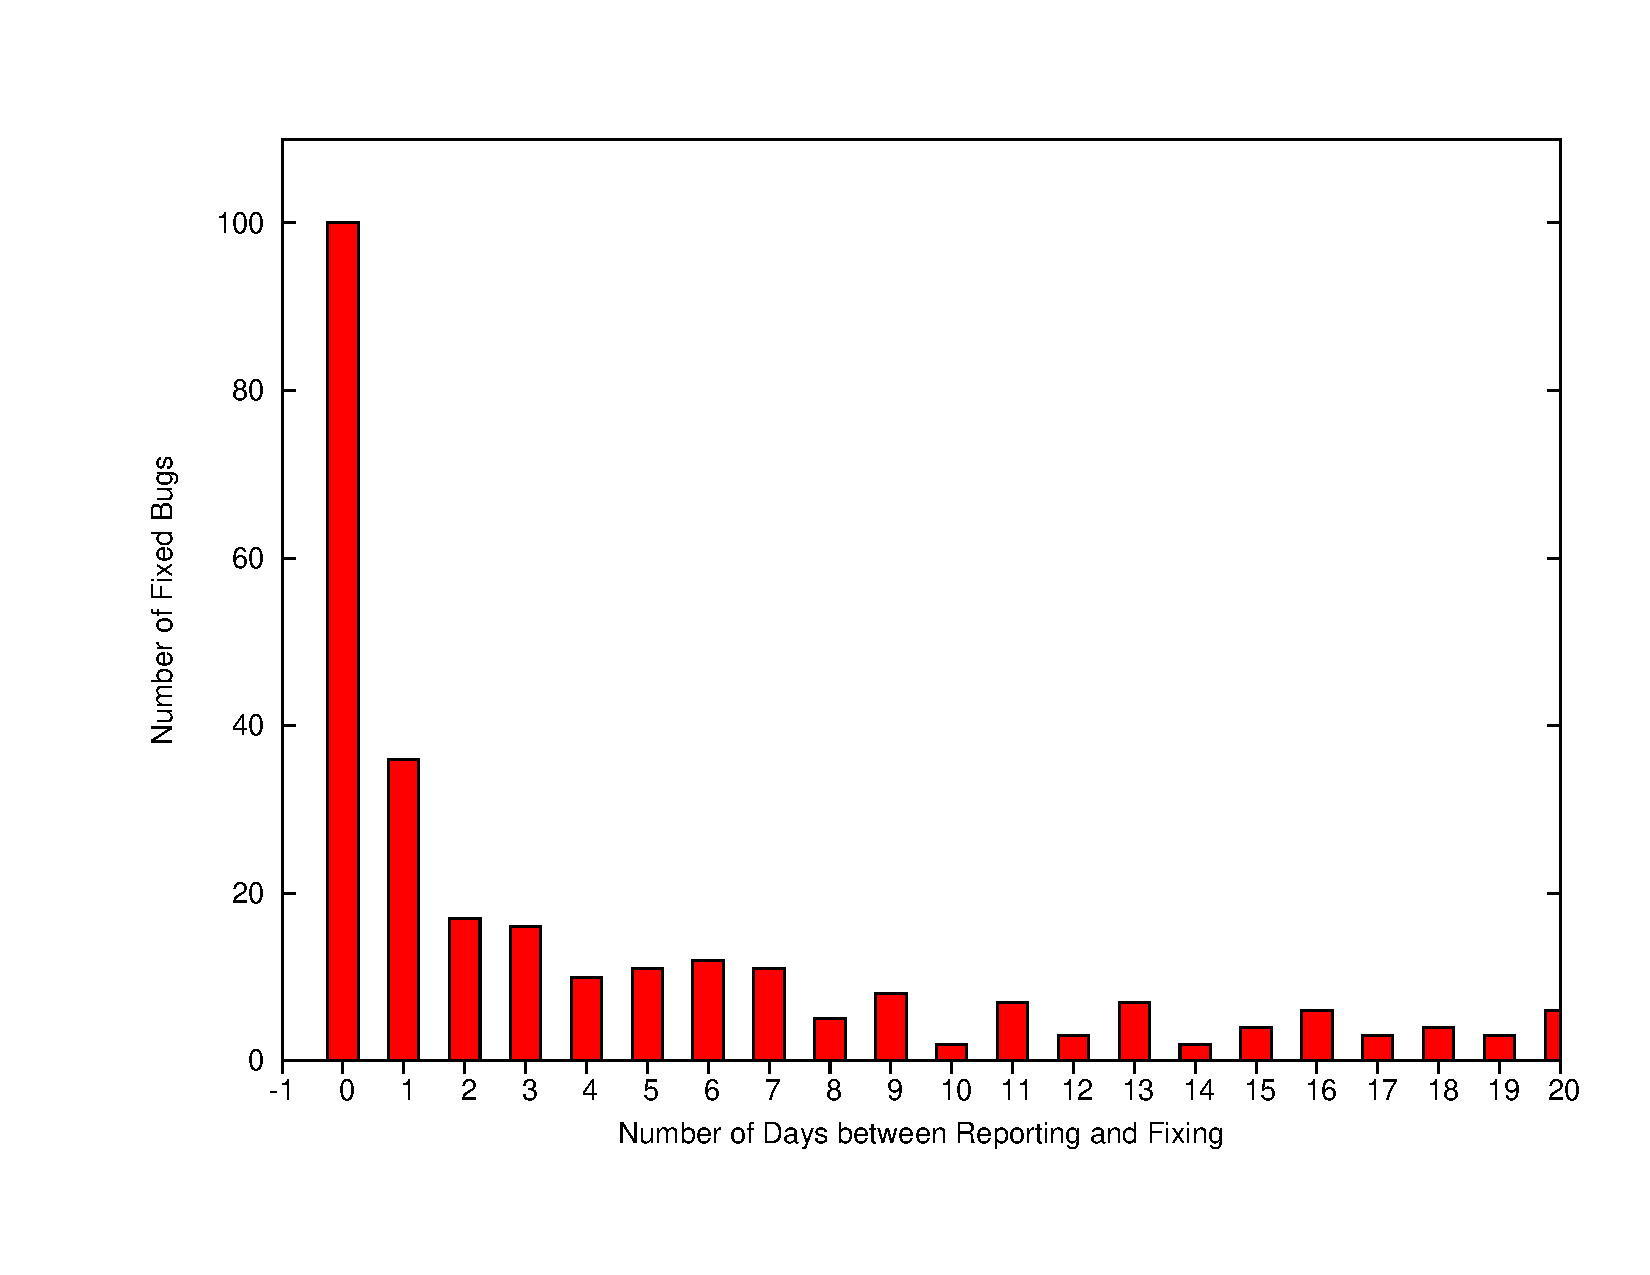
\includegraphics[width=0.9\textwidth,height=0.9\paperheight]{../Art/ITKBugFixesScheduleHistogramPlot.pdf}
\end{frame}


{
\setbeamertemplate{navigation symbols}{}
\setbeamertemplate{background canvas}{
  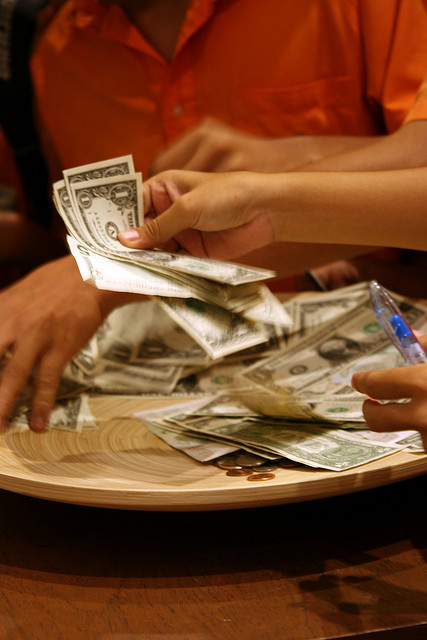
\includegraphics[width=0.55\textwidth,height=\paperheight]{../Art/2672465894_5b21e12135_z.jpg}
  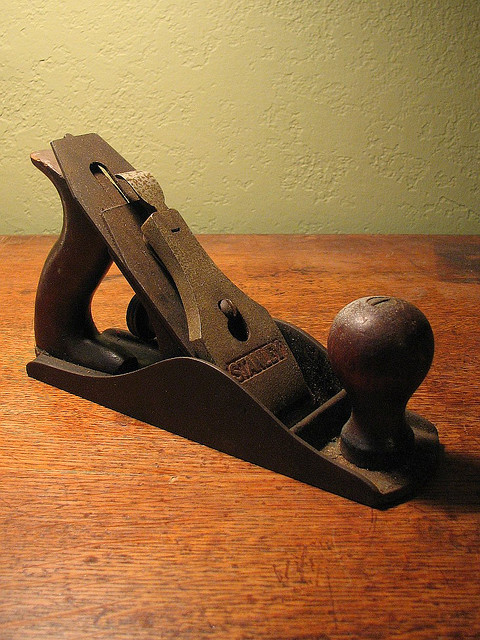
\includegraphics[width=0.55\textwidth,height=\paperheight]{../Art/4293485922_7474ef04ce_z.jpg}
  }
\begin{frame}
\frametitle{Bug/Issue Tracker}
\end{frame}
}


{
\setbeamertemplate{navigation symbols}{}
\setbeamertemplate{background canvas}{
  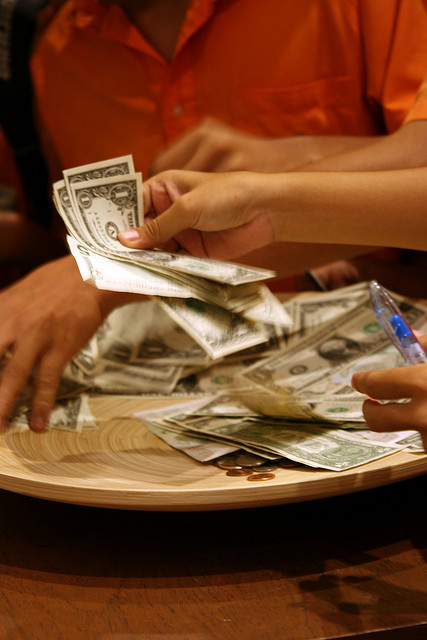
\includegraphics[width=0.55\textwidth,height=\paperheight]{../Art/2672465894_5b21e12135_z.jpg}
  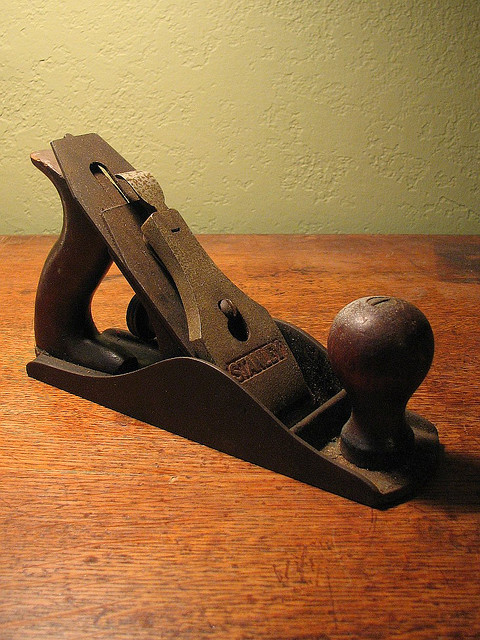
\includegraphics[width=0.55\textwidth,height=\paperheight]{../Art/4293485922_7474ef04ce_z.jpg}
  }
\begin{frame}
\frametitle{Wikis}
\end{frame}
}


{
\setbeamertemplate{navigation symbols}{}
\setbeamertemplate{background canvas}{
  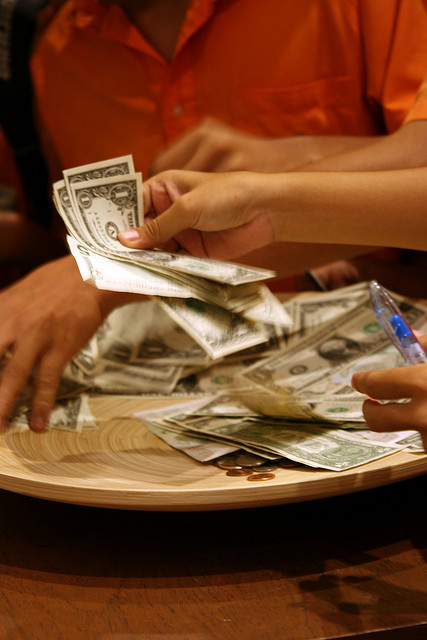
\includegraphics[width=0.55\textwidth,height=\paperheight]{../Art/2672465894_5b21e12135_z.jpg}
  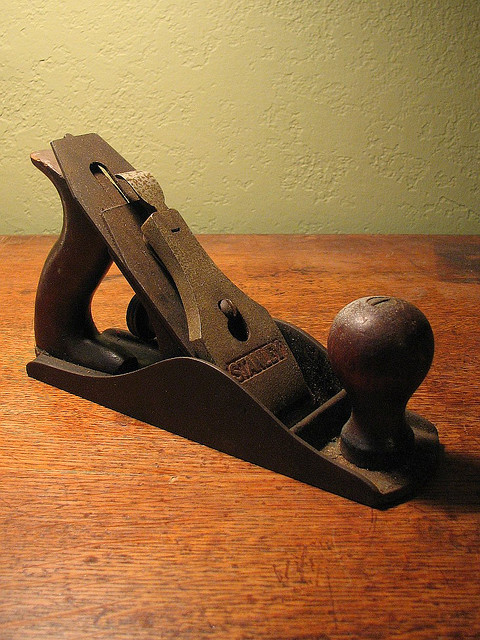
\includegraphics[width=0.55\textwidth,height=\paperheight]{../Art/4293485922_7474ef04ce_z.jpg}
  }
\begin{frame}
\frametitle{Phone Conferences}
\end{frame}
}


\begin{frame}
\frametitle{Code Repositories}
\Huge
\begin{itemize}
\item Backup
\pause
\item History of Changes
\pause
\item Collaboration Platform
\end{itemize}
\end{frame}


\begin{frame}
\frametitle{Code Repositories}
\Huge
\begin{itemize}
\item Who ?
\pause
\item What ?
\pause
\item When ?
\pause
\item \textbf{Why} ?
\end{itemize}
\end{frame}


\begin{frame}
\frametitle{Code Repositories}
\Huge
Typical Choices
\begin{itemize}
\item CVS
\pause
\item SVN
\pause
\item Git
\pause
\item Mercurial
\end{itemize}
\end{frame}


\begin{frame}
\frametitle{Code Repositories - Github}
\Huge
% FIXME Insert Github screenshot here
\end{frame}


\begin{frame}
\frametitle{Distributed Code Repositories}
\Huge
\begin{itemize}
\item Branching and Merging
\pause
\item Peripherial Development
\pause
\item Clean Releases
\end{itemize}
\end{frame}


\centeredlargetext{black}{white}{
Indirect Appropriation
}


\begin{frame}
\frametitle{Credits}
\begin{itemize}
\item \url{http://opensource.org/files/osi_standard_logo.png}
\item \url{http://www.flickr.com/photos/lifeontheedge/2672465894}
\item \url{http://www.flickr.com/photos/hortulus_aptus/4293485922}
\item \url{http://en.wikipedia.org/wiki/File:Iceberg_Antarctica.jpg}
\item \url{http://en.wikipedia.org/wiki/File:Iceberg.jpg}
\item \url{http://en.wikipedia.org/wiki/File:Hyundai_car_assembly_line.jpg}
\item \url{http://www.flickr.com/photos/spencer77/4924182750}
\item \url{http://www.zimbio.com/photos/Elinor+Ostrom/Nobel+Prize+Award+Ceremony+2009/quiD3nGLq-e}
\end{itemize}
\end{frame}


\begin{frame}
\frametitle{Credits}
\begin{itemize}
\item \url{http://www.flickr.com/photos/mwichary/2150546585}
\item \url{http://commons.wikimedia.org/wiki/File:Linus_Torvalds_lks08.jpg}
\item \url{http://en.wikipedia.org/wiki/File:Apples_supermarket.jpg}
\item \url{http://www.flickr.com/photos/amagill/3366720659}
\end{itemize}
\end{frame}


\end{document}
